\documentclass[main.tex]{subfiles}

\pagestyle{fancy}
%\fancyhf{}
\rhead{Assignment 4 - Multi-element Airfoil}
\lhead{AE4130 | 4738942}
\renewcommand{\headrulewidth}{0.1pt}
\begin{document}
\section{Problem Statement}
The aim of this assignment is two fold:to perform a literature study on high lift multi-element airfoils mainly using the Ref\cite{highliftaero} and \cite{van2002aerodynamic}. Based on the study, the main effects that determine the behaviour of high lift systems are elucidated. The second part involves numerical calculations for "like-wise" multi-element models and compare it with experimental data, using any 2D analysis code.
\section{Theory and Procedure}
The multi-element airfoils are used today to complement the need of high lift systems. Higher lift coefficients help in improving the the wing loading. Relatively high wing loading leads to increase in fuel efficiency in commercial aircrafts. Also, the critical STOL requirements can be attained through the use of such complex designs. High lift devices can in turn have a detrimental effect on cruise performance, in the form of additional parasitic drag. This report deals with the fundamentals as well as analysis of case specific multi-element high lift systems. The first portion explains the main effects that determine the behaviour of high lift systems, elucidated with hand-drawn sketches. This is followed by the construction and simulation of a high lift system using JavaFoil. The results are simultaneously compared with experimental data and observations reported, and this has been repeated for a plain flap as well. 
\subsection{The Slat Effect}
\textit{The velocities at the leading edge of the downstream element (main airfoil) are reduced due to the circulation of the upstream element (slat) thus reducing the pressure peaks of the downstream element.}\cite{slat} 
\\To understand the above statement lets consider a slat placed in front of an airfoil(main element/airfoil) as shown in the Figure \ref{fig1a}. The main purpose of the slat is to delay the angle of stall. At higher incidence angles, the suction pressure on the nose of the main airfoil drastically increases. This is to be decreased artificially. To do this, an additional lifting surface(in this case, a slat) is place in front of the main airfoil such that its wake vorticity becomes the upstream flow for the main airfoil. This is shown in Fig. 1. By doing this, the velocity vectors at the nose of the main airfoil are facing the opposite direction, than from an isolated airfoil. The result is a gradual pressure distribution without a flow separation until the trailing edge of the airfoil. This velocity distribution is shown in Figure \ref{fig1b}.
\begin{figure}[h!]
    \vspace*{-1.5em}\centering
    \subfloat[Wing section with LE slat]{
        \includegraphics[width=0.5\textwidth] {./Images/Ass4/Fig1_both}
        \label{fig1a} } \hspace*{-1.2em}
    \subfloat[Velocity Distribution]{
        \includegraphics[width=0.5\textwidth] {./Images/Ass4/Fig1b}
        \label{fig1b} } \\\vspace*{-0.5em}
    \caption{Slat Effect}
    \label{fig1}
\end{figure}
\\ The velocity distribution in Figure \ref{fig1b} is such that the peak suction pressure for the isolated airfoil has been countered by the clockwise vortex formation of the flow. The reported work of \textit{A.M.O.Smith, [1975]}\cite{highliftaero} also suggests that, if an identical-inverted-mirror image of the isolated airfoil suction pressure can be created for the vortex using a slat, then the suction pressure peak can be entirely cancelled. Studies also showed that the C$_L$ of the isolated airfoil to be greater than the main airfoil. But the combination of vortex and main airfoil resulted in a much higher C$_L$ than the isolated airfoil. This is exactly what the slat effect is meant to achieve.
\subsection{The Circulation Effect}
To understand the circulation effect, lets consider the use of TE flaps. Here the main airfoil will be upstream of the additional element. Similar to the previous case, here the vorticity is at the trailing edge of the main airfoil, is shown in Figure \ref{fig2a}. This places the trailing edge at a very high angle of attack. An important note is that here, the flow is not deflecting the flap(like in a normal flap), instead the vortex acts as a device which turns the flow. As a result, the circulation must increase inorder to satisfy the Kutta condition, thereby increasing the upper surface velocity over the upstream airfoil(see Figure \ref{fig2b}
\begin{figure}[h!]
    \vspace*{-1.5em}\centering
    \subfloat[Wing section with flap(shown as point vortex)]{
        \includegraphics[width=0.4\textwidth] {./Images/Ass4/Fig2a}
        \label{fig2a} } \hspace*{-1.2em}
    \subfloat[Velocity Distribution]{
        \includegraphics[width=0.5\textwidth] {./Images/Ass4/Fig2b}
        \label{fig2b} } \\\vspace*{-0.5em}
    \caption{Circulation Effect}\vspace*{-1.9em}
    \label{fi2g2}
\end{figure}

\subsection{The Dumping Effect} \label{dump}
The dumping effect is a consequence of the circulation effect, due to the additional velocity caused by adding the vortex, the airfoil discharges a boundary layer at the TE into a stream that is at a higher velocity. i.e. the BL of the upstream element gets dumped into this zone. This leads to decreases in the need of pressure recovery, thereby increasing the lift. 
\begin{figure}[h!]
\vspace*{-0.5em}\centering
\includegraphics[width=0.6\textwidth]{./Images/Ass4/Fig4}\vspace*{-1.3em}
\caption{Increased Velocity at TE of main airfoil due to dumping affect}\vspace*{-0.5em}
\label{Fig4}
\end{figure}\vspace*{-1.0em}

\subsection{Off-the-Surface Pressure Recovery}
As a result of the dumping effect, the flow stream in the boundary layer exits the TE of the multi-element airfoil at a higher velocity than free stream. The recovery back to free stream velocity can be more efficient away from the wall. If the flow tries to achieve free stream velocity close to the wall, then the pressure recovery is adversely affected.    

\subsection{The Fresh Boundary Layer Effect}
The fact that every consecutive addition of an element in an airfoil will lead to formation of multiple boundary layers, each one leading to lesser pressure recovery demands. The TE velocity of each element is relatively higher leading to a thinner BL than the upstream element. As mentioned by \textit{A.M.O.Smith, [1975]}\cite{highliftaero}, thinner boundary layers can sustain greater pressure gradients than thicker ones. This also why off-the-surface pressure recovery is so beneficial, since flow decelerates away from the wall.
\pagebreak
\section{Results and Discussion}

\subsection{Comparison of Slotted Flap with Exp. Data}
Now that we have seen the five main effects that can be exploited to create a high lift system, an external slotted flap airfoil was created. The NACA 23012 was chosen for this, since extensive experimental data for various flap settings were available directly. In order to replicate the experimental data\cite{wenzinger1939wind}, NACA 23012 is used for both the main airfoil and the external flap. Four different flap delfection($\delta_f$) settings have been compared for this external flap, \{$-2.5^{\circ},10.2^{\circ},20.2^{\circ},30.2^{\circ}$\}. The scaling of the flap and main airfoil was performed according to the procedure in Ref.\cite{wenzinger1939wind}. The boundary conditions chosen for the analysis and the profiles of the airfoils are shown in Table \ref{table1}. and Figure 4 respectively.
\begin{table}[h]\begin{center}\begin{tabular}{ c c } 
 \hline \rowcolor{lightgray}
  \hspace{0.5cm}Quantity\hspace{0.5cm} & \hspace{0.5cm}Value\hspace{0.5cm} \\
  \hline
  $\alpha$ & [-8:16]\\
 \hline
  $\delta$ & \{$-2.5^{\circ},10.2^{\circ},20.2^{\circ},30.2^{\circ}$\}\\
 \hline
  R$_e$ & $3.5\times10^6$  \\ 
   \hline
  Mach & 0.0  \\ 
   \hline
  Stall Model & CalcFoil \\ 
 \hline
 Transition Model & Drela e$^N$\\
\hline
\end{tabular}\caption{BCs used for JavaFoil$\textregistered$ simulation}\vspace*{-2em}\label{table1}\end{center}\end{table}

\begin{figure}[h!]
    \vspace*{-1em}\centering
    \hspace*{-1.5em}\subfloat[Wing section with flap(shown as point vortex)]{
        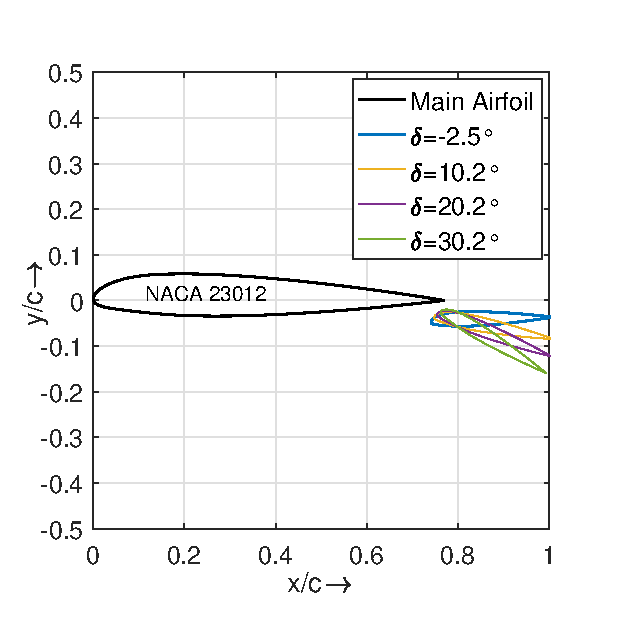
\includegraphics[width=0.55\textwidth] {./Images/Ass4/Airfoil_ExternalFlap}
        \label{fig4a} } \hspace*{-1.2em}
    \subfloat[Velocity Distribution]{
        \includegraphics[width=0.5\textwidth] {./Images/Ass4/Ref_ExternalFlap}
        \label{fig4b} } \\\vspace*{-0.5em}
    \caption{NACA 23012 with slotted flap at various flap deflections}
    \label{fig4}
\end{figure}
\pagebreak
\\\noindent Figure \ref{fig5} shows the comparison of the coefficient of lift at 4 different flap settings. The thin dotted lines represent the results from this analysis, the thicker lines are the corresponding experimental data taken from Ref\cite{wenzinger1939wind}.

\begin{figure}[h!]
\centering
\hspace{1.8cm}\includegraphics[width=0.65\textwidth]{./Images/Ass4/Cl_Comparison}
\caption{Lift Polar comparison between JAVAFOIL simulation and experimental data}
\label{fig5}
\end{figure}
At lower flap deflection angles of \{$-2.5^{\circ},10.2^{\circ}$\} the simulation results were in more agreement than at  \{$20.2^{\circ},30.2^{\circ}$\}. At higher incidence angles of the overall multi-element system, the simulation results starts to diverge from the experimental data. Different transition models were studied, finally the $Drela$ $e^N$ approximation was used. The poor identification of laminar separation region and transition point in JAVAFOIL could be responsible for this diverging behaviour. At higher flap deflections, the C$_L$ is approximately 45\% higher than experimental data. The fact that this has been observed for lower incidence angles, could be because of the potential flow assumtions in JAVAFOIL.\\ 

\vspace{0.35cm}\begin{tcolorbox}[colback=gray!5!white,colframe=gray!75!black]
\textit{In JAVAFOIL there is no interaction between the boundary layer and the external flow, as in XFOIL, though. Therefore largely separated flows cannot be analyzed – a short flow separation ( $s_{seperated}/c < 10\% $) at the trailing edge does not affect the results very much. Also laminar separation bubbles are not modeled; when laminar separation is detected the code switches to turbulent flow.}
\label{JAVAFOIL}
\end{tcolorbox}
\vspace{0.35cm}
\\The JAVAFOIL User Manual\cite{JAVAFOIL_User_Guide} itself states why such discrepancies may arise at stall angles. Figure \ref{fig6} shows the streamlines in a pressure contour for one combination of angle of attack and flap deflection. The LE suction peak can be visualized on the main airfoil. The flap, despite having the exact airfoil has more of a steady pressure gradient. This is because of the Dumping Effect\ref{dump} and the BL effects seen before. From a simulation perspective the streamlines look smooth, but at such high angles of attack flow separation is expected. This is not observed, neither is the wake region behind the airfoil captured properly. This is because of the primitive nature of JAVAFOIL's flow analysis model. The proposed JAVAFOIL application seems to under-predict certain well studied boundary layer effects, especially the laminar separation bubbles. The model simply switches to turbulent flow behavior when it encounters the flow separation criteria. Also, the solver uses vorticity distribution to solve the flowfield using a primitive boundary layer method and neglects friction. Due to these reasons the proposed prediction model will not be used in future tasks. But the easy use of the multi-element module and its satisfactory results, makes it a good first level approximation for future high lift airfoil analysis. \\

\begin{figure}[t]
\centering
\includegraphics[width=1\textwidth]{./Images/Ass4/Alpha6_FlapDef10_2_Contours}
\caption{Pressure contours around NACA23012 with external flap at $\alpha=6^{\circ}$ $\delta=10.2^{\circ}$}
\label{fig6}
\end{figure}

\subsection{Comparison of External Flap with Plain Flap}
JAVAFOIL applet is used for the comparative study between a plain flap and external Flap. The flow BCs and analysis parameters from Table \ref{table1} is used in this study. The plain flap and the slotted flap show similar lift coefficients. At higher flap deflections positions, the external flap is performing slightly better than the plain flap. Although the slotted external flap is expected to perform better, a noteworthy deviation is not observed from these JAVAFOIL results. But what can be said is that, the the plain flap does not have any slots downstream, the external flap takes advantage of the circulation effect in order to produce lift, as explained in previous sections. Moreover, the plain flaps do not allow for the regeneration of the boundary layer at the flap leading edge. This leads to loss in terms of separation. The modelling assumptions of JAVAFOIL again fail at calculating this correctly.
\pagebreak
\begin{figure}[h!]
\centering
\includegraphics[width=0.9\textwidth]{./Images/Ass4/AllFlap_Comparison}
\caption{Lift Polar comparison between Plain and Slotted flap, with Experimental datas}
\label{fig7}
\end{figure}

\\\noindent For the theoretical calculation and comparison, the following equation is used\cite{irving1976synthesis};

\begin{equation}
    (\Delta C_l)_{th} = \frac{2\pi}{57.3}\left(1+0.77\frac{t}{c}\right)a_{\delta}\delta_f
\end{equation}
\vspace{-0.5cm}\begin{align*}
\centering
\begin{split}
    a_\delta \longrightarrow {}& Theoretical\ flap\ li\!ft\ factor\\
\end{split}\\
\begin{split}
    \delta_f \longrightarrow {}& Flap\ angle\\
\end{split}\\
\begin{split}
    t/c \longrightarrow {}& Thickness\ to\ chord\ of\ main\ air\!foil\\
\end{split}\\
\end{align*}
\pagebreak
\begin{table}[t]\begin{center}\begin{tabular}{ c c } 
 \hline \rowcolor{lightgray}
  \hspace{0.5cm}$\delta_f[^{\circ}]$\hspace{0.5cm} & \hspace{0.5cm}$(\Delta C_l)_{th}$\hspace{0.5cm} \\
  \hline
  -2.5 & 0.164\\
 \hline
  10.2 & 0.671\\
 \hline
  20.2 & 1.329\\ 
   \hline
 30.2 & 1.987 \\ 
\hline
\end{tabular}\caption{Theoretical lift calculations for external flap}\vspace*{-2em}\label{table2}\end{center}\end{table}
\\\noindent Using this formula, the theoretical lift is determined and tabulated in Table \ref{table2}. The theoretical calculations are a better approximation only at higher flap angles. But due to the linear nature of the equation, this result is meaningful and valid only in a narrow bracket of flap deflections.


\printbibliography[title={References}]
\end{document}
